\documentclass[12pt]{article}
\usepackage[dvips]{graphicx}
\topmargin -40pt
\headsep 30pt
\evensidemargin 0pt
\oddsidemargin 0pt
\textwidth 490pt
\textheight 650pt


\def\beq{\begin{equation}}
\def\eeq{\end{equation}}

\begin{document}

%\newpage
\section*{Verdict Hexahedral Metrics:}

\subsection*{Variable Definitions:}

\begin{figure}[htb]
  \begin{center}
    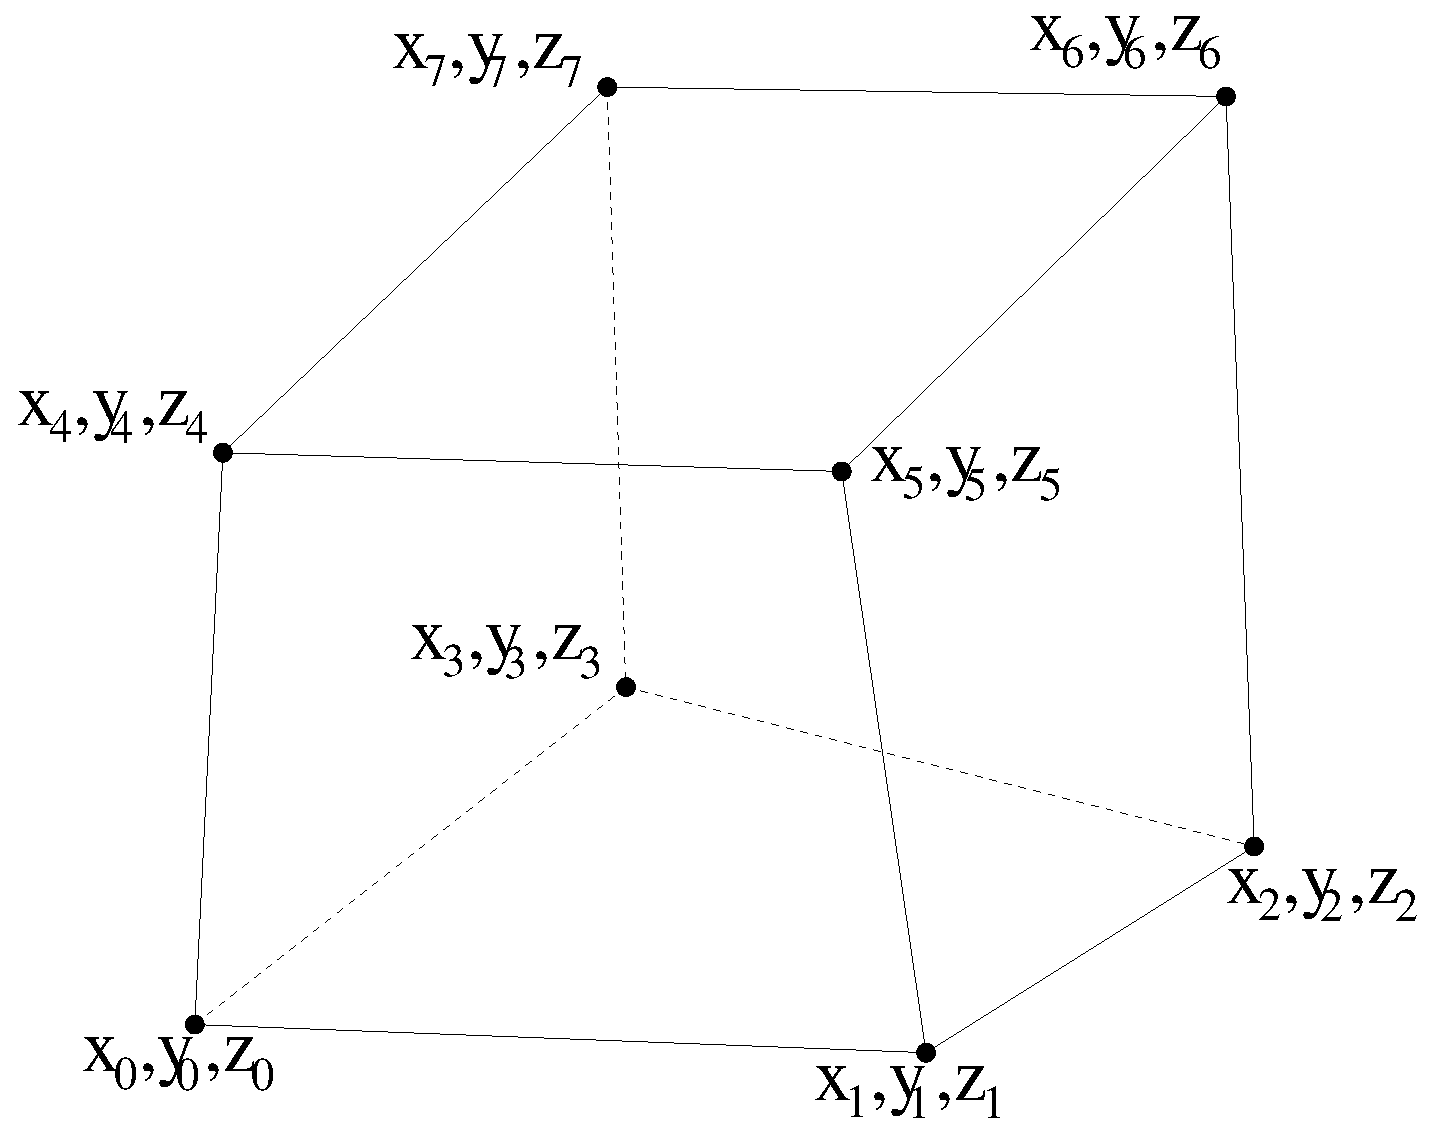
\includegraphics[height=2.0in]{hex.eps}
    \caption{Vertices of Hexahedron}
    \label{fig:blank}
  \end{center}
\end{figure}

\subsubsection*{Hex Vertices:}
\begin{center}
$\vec P_0 = (x_0, y_0, z_0)$ 
\end{center}

\begin{center}
$\vec P_1 = (x_1, y_1, z_1)$ 
\end{center}

\begin{center}
$\vec P_2 = (x_2, y_2, z_2)$
\end{center}

\begin{center}
$\vec P_3 = (x_3, y_3, z_3)$ 
\end{center}

\begin{center}
$\vec P_4 = (x_4, y_4, z_4)$ 
\end{center}

\begin{center}
$\vec P_5 = (x_5, y_5, z_5)$
\end{center}

\begin{center}
$\vec P_6 = (x_6, y_6, z_6)$ 
\end{center}

\begin{center}
$\vec P_7 = (x_7, y_7, z_7)$ 
\end{center}

\subsubsection*{Hex Edges:}

\begin{center}
$\vec L_0 = \vec P_1 - \vec P_0 $
\end{center}

\begin{center}
$\vec L_1 = \vec P_2 - \vec P_1 $
\end{center}

\begin{center}
$\vec L_2 = \vec P_3 - \vec P_2 $
\end{center}

\begin{center}
$\vec L_3 = \vec P_3 - \vec P_0 $
\end{center}

\begin{center}
$\vec L_4 = \vec P_4 - \vec P_0 $
\end{center}

\begin{center}
$\vec L_5 = \vec P_5 - \vec P_1 $
\end{center}

\begin{center}
$\vec L_6 = \vec P_6 - \vec P_2 $
\end{center}

\begin{center}
$\vec L_7 = \vec P_7 - \vec P_3 $
\end{center}

\begin{center}
$\vec L_8 = \vec P_5 - \vec P_4 $
\end{center}

\begin{center}
$\vec L_9 = \vec P_6 - \vec P_5 $
\end{center}

\begin{center}
$\vec L_{10} = \vec P_7 - \vec P_6 $
\end{center}

\begin{center}
$\vec L_{11} = \vec P_7 - \vec P_4 $
\end{center}

\begin{center}
$L_{min} = MIN\left(| \vec L_0 |,| \vec L_1|, .... |\vec L_{11}| \right) $
\end{center}

\subsubsection*{Hex Diagonals:}

\begin{center}
$\vec D_0 = \vec P_6 - \vec P_0 $
\end{center}

\begin{center}
$\vec D_1 = \vec P_7 - \vec P_1 $
\end{center}

\begin{center}
$\vec D_2 = \vec P_4 - \vec P_2 $
\end{center}

\begin{center}
$\vec D_3 = \vec P_5 - \vec P_3 $
\end{center}

\begin{center}
$D_{min} = MIN\left( | \vec D_0|, |\vec D_1|, |\vec D_2|, |\vec D_3| \right) $
\end{center}
\begin{center}
$D_{max} = MAX\left( | \vec D_0|, |\vec D_1|, |\vec D_2|, |\vec D_3| \right) $
\end{center}

\subsubsection*{Principal Axes:}

\begin{center}
$\vec X_1 = -\vec P_0 - \vec P_3 - \vec P_4 - \vec P_7 
            +\vec P_1 + \vec P_2 + \vec P_5 + \vec P_6$
\end{center}

\begin{center}
$\vec X_2 = -\vec P_0 - \vec P_1 - \vec P_4 - \vec P_5 
            +\vec P_2 + \vec P_3 + \vec P_6 + \vec P_7$
\end{center}

\begin{center}
$\vec X_3 = -\vec P_0 - \vec P_1 - \vec P_2 - \vec P_3 
            +\vec P_4 + \vec P_5 + \vec P_6 + \vec P_7$
\end{center}

\subsubsection*{Cross Derivatives:}

\begin{center}
$\vec X_{23} = \vec P_0 + \vec P_1 + \vec P_6 + \vec P_7 
          - \vec P_2 - \vec P_3 - \vec P_4 - \vec P_5$
\end{center}

\begin{center}
$\vec X_{13} = \vec P_0 + \vec P_3 + \vec P_5 + \vec P_6 
          - \vec P_1 - \vec P_2 - \vec P_4 - \vec P_7$
\end{center}

\begin{center}
$\vec X_{12}= \vec P_0 + \vec P_2 + \vec P_4 + \vec P_6 
          - \vec P_1 - \vec P_3 - \vec P_5 - \vec P_7$
\end{center}

\subsubsection*{Hex Matrices:}

\begin{center}
$A_0 = [ \vec L_0, \vec L_3, \vec L_4 ]$
\end{center}

where $\vec L_0$, $\vec L_3$, and $\vec L_4$ form the columns of $A_0$, etc.

\begin{center}
$A_1 = [ \vec L_1, -\vec L_0, \vec L_5 ]$
\end{center}

\begin{center}
$A_2 = [ \vec L_2, -\vec L_1, \vec L_6 ]$
\end{center}

\begin{center}
$A_3 = [ -\vec L_3, -\vec L_2, \vec L_7 ]$
\end{center}

\begin{center}
$A_4 = [ \vec L_{11}, \vec L_8, -\vec L_4 ]$
\end{center}

\begin{center}
$A_5 = [ -\vec L_8, \vec L_9, -\vec L_5 ]$
\end{center}

\begin{center}
$A_6 = [ -\vec L_9, \vec L_{10}, -\vec L_6 ]$
\end{center}

\begin{center}
$A_7 = [ -\vec L_{10}, -\vec L_{11}, -\vec L_7 ]$
\end{center}

\begin{center}
$A_8 = [ \vec X_1, \vec X_2, \vec X_3 ]$
\end{center}

\subsection*{Matrix Operations:}

Let $A$ be a $3 \times 3$ matrix defined by the column vectors $\vec v_1, \vec v_2, \vec v_3,$ i.e., $A = [\vec v_1, \vec v_2, \vec v_3]$. 

\begin{flushleft}
Then, 
\end{flushleft}

\begin{displaymath}
|A|^2 = |\vec v_1|^2 + |\vec v_2|^2 + |\vec v_3|^2 
\end{displaymath}

\begin{displaymath}
|adj(A)|^2 = |\vec v_1 \times \vec v_2|^2 + 
             |\vec v_2 \times \vec v_3|^2 +
             |\vec v_3 \times \vec v_1|^2  
\end{displaymath}

\begin{displaymath}
\alpha = determinant(A) = \vec v_1 \cdot (\vec v_2 \times \vec v_3 )
\end{displaymath}

\begin{displaymath}
\alpha_k = determinant(A_k) ~ where ~ k=0,1,...,8
\end{displaymath}

\begin{displaymath}
\hat{A} = \left[ \frac {\vec v_1} {|v_1|}, 
                 \frac {\vec v_2} {|v_2|},
                 \frac {\vec v_3} {|v_3|} \right] 
\end{displaymath}

\begin{displaymath}
\hat \alpha_k = determinant(\hat A_k) ~ where ~ k=0,1,...,8
\end{displaymath}

\subsection*{Overflow:}

\begin{flushleft}
The metrics below are all checked for overflow like so:
\end{flushleft}

\begin{flushleft}
\quad ${IF \quad metric\_value > 0;  \quad metric\_value = MIN( metric\_value, DBL\_MAX )}$
\end{flushleft}
 
\begin{flushleft}
\quad ${ELSE \quad metric\_value = MAX( metric\_value, -DBL\_MAX )}$
\end{flushleft}
 
\subsection*{Metric Ranges:}

\begin{flushleft}
Acceptable Range: Well-behaved elements will have metrics in this range.
\end{flushleft}
\begin{flushleft}
Normal Range:     All elements except those with degeneracies will have  \newline
                  metrics in this range.
\end{flushleft}
\begin{flushleft}
Full Range:       All elements including degenerate ones will have metrics \newline
                  in this range. 
\end{flushleft}

%---------------------------Aspect Ratio---------------------------
\subsection*{Hex Aspect Ratio:}

\begin{displaymath}
aspect_{12} = \frac{ MAX \left( \left| \vec X_1 \right|,  \left| \vec X_2 \right|  \right) } 
                    { MIN \left( \left| \vec X_1 \right|,  \left| \vec X_2 \right|  \right) }
\end{displaymath}

\begin{displaymath}
aspect_{13} = \frac{ MAX \left( \left| \vec X_1 \right|,  \left| \vec X_3 \right|  \right) } 
                    { MIN \left( \left| \vec X_1 \right|,  \left| \vec X_3 \right|  \right) } 
\end{displaymath}

\begin{displaymath}
aspect_{23} = \frac{ MAX \left( \left| \vec X_2 \right|,  \left| \vec X_3 \right|  \right) } 
                    { MIN \left( \left| \vec X_2 \right|,  \left| \vec X_3 \right|  \right) } 
\end{displaymath}

\begin{center}
$aspect = MAX\left( aspect_{12}, aspect_{13}, aspect_{23} \right)$
\end{center}

\begin{tabular}{lll}
& Metric Description:  & Maximum pairwise length ratio between principle axes. \\
& Dimension:           & $L^0$       \\ 
& Acceptable Range:    & 1 to 1.3               \\ 
& Normal Range:        & 1 to $DBL\_MAX$                      \\ 
& Full Range:          & 1 to $DBL\_MAX$ \\ 
& Value of Metric on Unit Cube:    & 1.0 \\
& Note:                & If $|\vec X_1 |$ or $|\vec X_2 |$ or $|\vec X_3| < DBL\_MIN$, \\
&                      & $aspect = DBL\_MAX$ \\
& Reference:           & Adapted from \cite{one} \\
\end{tabular} 


%---------------------------Condition---------------------------
\subsection*{Hex Condition:}

\begin{displaymath}
\kappa(A) = |A| |A^{-1}| = \frac {|A| |adj(A)|} {\alpha}
\end{displaymath}

\begin{center}
$condition~number = \frac {1}{3} MAX( \kappa(A_0), \kappa(A_1), .....\kappa(A_8))$
\end{center}

\begin{tabular}{lll}
& Metric Description:  & Maximum condition number of the Jacobian matrix at  \\
&                      & 8 corners and center.\\ 
& Dimension:           & $L^0$       \\ 
& Acceptable Range:    & 1 to 3               \\ 
& Normal Range:        & 1 to $DBL\_MAX$                      \\ 
& Full Range:          & 1 to $DBL\_MAX$ \\ 
& Value of Metric on Unit Cube:    & 1.0 \\
& Note:                & If $\alpha_k \leq DBL\_MIN$, for any $k$, $condition = DBL\_MAX$\\ 
& Reference:           & \cite{three} \\
\end{tabular} 


%---------------------------Diagonal---------------------------
\subsection*{Hex Diagonal:}

\begin{displaymath}
diagonal = \frac {D_{min}} { D_{max}} 
\end{displaymath}

\begin{tabular}{lll}
& Metric Description:  & Ratio of minimum to maximum diagonal. \\ 
& Dimension:           & $L^0$                              \\ 
& Acceptable Range:    & 0.65 to 1  \\
& Normal Range:        & 0 to 1 \\ 
& Full Range:          & 0 to $DBL\_MAX$ \\ 
& Value of Metric on Unit Cube:    & 1.0 \\
& Note:                & If $D_{max} < DBL\_MIN$, $diagonal = DBL\_MAX $ \\ 
& Reference:           & Unknown \\ 
\end{tabular} 


%---------------------------Distortion---------------------------
\subsection*{Hex Distortion:} 

\begin{displaymath}
distortion = \frac{ |J|*master\textrm{-}volume} { true\textrm{-}volume }  
\end{displaymath}

\begin{flushleft} Where, \end{flushleft}
$|J| = $ minimum determinant of the Jacobian computed over all Gauss points  \newline
of the element.  The location of the Gauss points is not documented. \newline 
$master\textrm{-}volume =$ volume of the master hex, where the master hex's corner \newline
nodes are as follows: \newline

 $\vec P_0 = (-1, -1, 0)$,  
 $\vec P_1 = (1, -1, 0)$,
 $\vec P_2 = (1, 1, 0)$, 
 $\vec P_3 = (-1, 1, 0)$  \newline

 $\vec P_4 = (-1, -1, 1)$,  
 $\vec P_5 = (1, -1, 1)$,
 $\vec P_6 = (1, 1, 1)$, 
 $\vec P_7 = (-1, 1, 1)$   \newline

\begin{tabular}{lll}
& Metric Description:  & Minimum Gauss Point Jacobian divided by hex \\
&                      & volume, times master hex's volume. \\ 
& Dimension:           & $L^3$       \\ 
& Acceptable Range:    & 0.5 to 1 \\ 
& Normal Range:        & 0 to 1 \\ 
& Full Range:          & $-DBL\_MAX$ to $DBL\_MAX$ \\ 
& Value of Metric on Unit Cube:    & 1.0 \\
& Note:                & This metric is currently unsupported. \\ 
& Reference:           & Adapted from \cite{five} \\
\end{tabular} 

%---------------------------Jacobian---------------------------
\subsection*{Hex Jacobian:}

\beq
jacobian = MIN\left( \alpha_0, \alpha_1, ...\alpha_7, \frac{\alpha_8} {64} \right)
\eeq

\begin{tabular}{lll}
& Metric Description:  & Minimum pointwise volume of local map at 8 corners \\ 
&                      & and center of hex. \\
& Dimension:           & $L^3$       \\ 
& Acceptable Range:    & 0 to $DBL\_MAX$ \\ 
& Normal Range:        & 0 to $DBL\_MAX$ \\ 
& Full Range:          & $-DBL\_MAX$ to $DBL\_MAX$ \\ 
& Value of Metric on Unit Cube:    & 1.0 \\
& Reference:           & \cite{three} \\
\end{tabular} 


%---------------------------Oddy---------------------------
\subsection*{Hex Oddy:}

\begin{displaymath}
O(A) = \frac {| A^t A |^2 - \frac {1}{3} | A |^4 } {(\alpha)^{ \frac {4}{3}}}
\end{displaymath}

\begin{center}
$oddy = MAX( O(A_0), O(A_1), ... O(A_8) )$
\end{center}

\begin{tabular}{lll}
& Metric Description:  & Maximum deviation of metric tensor ($A^t A$) at hex \\
&                      & corners and center from identity matrix.\\ 
& Dimension:           & $L^0$       \\ 
& Acceptable Range:    & 0 to 0.5 \\ 
& Normal Range:        & 0 to $DBL\_MAX$ \\ 
& Full Range:          & 0 to $DBL\_MAX$ \\
& Value of Metric on Unit Cube:    & 0.0 \\
& Note:                & if $\alpha_k \leq DBL\_MIN$ for any $k$, $oddy = DBL\_MAX$ \\ 
& Reference:           & Adapted from \cite{six} \\
\end{tabular} 


%---------------------------Relative Size Squared---------------------------
\subsection*{Hex Relative Size-Squared:}

\begin{displaymath}
D = {\frac {\sum_{i=0}^7 \alpha_i} {8*Average~Hex~Volume}} 
\end{displaymath}

\begin{displaymath}
relative~size \textrm{-}squared = {MIN( D, \frac {1}{D})}^2 
\end{displaymath}

\begin{flushleft}
$Average ~ Hex ~ Volume$ is the average volume of the hexes in the \\
group of hexes being analyzed. \\
\end{flushleft}

\begin{tabular}{lll}
& Metric Description:  & Square of minimum of the ratio of hex volume to  \\
&                      & average hex volume and the inverse ratio.\\
& Dimension:           & $L^0$       \\ 
& Acceptable Range:    & 0.5 to 1 \\ 
& Normal Range:        & 0 to 1 \\ 
& Full Range:          & 0 to 1 \\ 
& Note:                & If $Average~Hex~Volume < DBL\_MIN$, $relative~size \textrm{-}squared = 0$ \\ 
&                      & If $D \leq DBL\_MIN$, $relative~size \textrm{-}squared = 0$ \\ 
& Reference:           & \cite{four} \\
\end{tabular} 


%---------------------------Scaled Jacobian---------------------------
\subsection*{Hex Scaled Jacobian:}

\begin{displaymath}
scaled~jacobian = MIN \left( \hat \alpha_0,
                             \hat \alpha_1,...,
                             \hat \alpha_8 \right)
\end{displaymath}

\begin{tabular}{lll}
& Metric Description:  & Minimum local Jacobian determinant divided by the \\ 
&                      & corresponding edge-lengths. \\
& Dimension:           & $L^0$       \\ 
& Acceptable Range:    & 0.5 to 1 \\ 
& Normal Range:        & -1 to 1 \\ 
& Full Range:          & -1 to $DBL\_MAX$ \\ 
& Value of Metric on Unit Cube:    & 1.0 \\
& Note:                & If ${L_{min}}^2 \leq DBL\_MIN$, $scaled~jacobian = DBL\_MAX$ \\ 
& Reference:           & \cite{three} \\
\end{tabular} 


%---------------------------Shape---------------------------
\subsection*{Hex Shape:}

\begin{displaymath}
shape = 3*MIN \left( \frac {{\alpha_0}^{\frac {2}{3}}} {|A_0|^2}, 
                     \frac {{\alpha_1}^{\frac {2}{3}}} {|A_1|^2},..., 
                     \frac {{\alpha_8}^{\frac {2}{3}}} {|A_7|^2} \right)
\end{displaymath}


\begin{tabular}{lll}
& Metric Description:  & 3/Mean Ratio of Jacobian matrix. \\ 
& Dimension:           & $L^0$       \\ 
& Acceptable Range:    & 0.3 to 1 \\ 
& Normal Range:        & 0 to 1 \\ 
& Full Range:          & 0 to 1 \\ 
& Value of Metric on Unit Cube:    & 1.0 \\
& Note:                & If $\alpha_k \leq DBL\_MIN$ for any $k$, $shape = 0$ \\ 
&                      & If $|A_k|^2 \leq DBL\_MIN$ for any $k$, $shape = 0$ \\ 
& Reference:           & \cite{four} \\
\end{tabular} 


%---------------------------Shape and Size---------------------------
\subsection*{Hex Shape and Size:}

\begin{displaymath}
shape~and~size = shape * relative~size \textrm{-}squared 
\end{displaymath}

\begin{tabular}{lll}
& Metric Description:  & Product of Shape and Relative Size.\\ 
& Dimension:           & $L^0$       \\ 
& Acceptable Range:    & 0.2 to 1 \\ 
& Normal Range:        & 0 to 1 \\ 
& Full Range:          & 0 to 1 \\ 
& Value of Metric on Unit Cube:    & 1.0 \\
& Reference:           & \cite{four} \\
\end{tabular} 


%---------------------------Shear---------------------------
\subsection*{Hex Shear:}

\begin{displaymath}
shear = MIN \left( {\hat \alpha_0},
                   {\hat \alpha_1},...,
                   {\hat \alpha_8} \right)
\end{displaymath}

\begin{tabular}{lll}
& Metric Description:  & Minimum Jacobian divided by product of lengths of 3 \\ 
&                      & edge vectors. \\
& Dimension:           & $L^0$       \\ 
& Acceptable Range:    & 0.3 to 1 \\ 
& Normal Range:        & 0 to 1 \\ 
& Full Range:          & 0 to 1 \\ 
& Value of Metric on Unit Cube:    & 1.0 \\
& Note:                & If $\hat \alpha_k \leq DBL\_MIN$ for any k, $shear = 0$ \\ 
&                      & If ${L_{min}}^2 \leq DBL\_MIN; shear = 0$ \\
& Reference:           & \cite{four} \\
\end{tabular} 


%---------------------------Shear and Size---------------------------
\subsection*{Hex Shear and Size:}

\begin{displaymath}
shear~and~size = shear * relative~size \textrm{-}squared 
\end{displaymath}

\begin{tabular}{lll}
& Metric Description:  & Product of Shear and Relative Size-Squared.\\ 
& Dimension:           & $L^0$       \\ 
& Acceptable Range:    & 0.2 to 1 \\ 
& Normal Range:        & 0 to 1 \\ 
& Full Range:          & 0 to 1 \\ 
& Value of Metric on Unit Cube:    & 1.0 \\
& Reference:           & \cite{four} \\
\end{tabular} 


%---------------------------Skew---------------------------
\subsection*{Hex Skew:}

\begin{displaymath}
\hat{X_1} = \frac {\vec X_1} {\left| \vec X_1 \right| }
\end{displaymath}

\begin{displaymath}
\hat{X_2} = \frac {\vec X_2} {\left| \vec X_2 \right| }
\end{displaymath}

\begin{displaymath}
\hat{X_3} = \frac {\vec X_3} {\left| \vec X_3 \right| }
\end{displaymath}

\begin{center}
$skew_{12} = \left| \hat{X_1} \cdot \hat{X_2} \right|$
\end{center}

\begin{center}
$skew_{13} = \left| \hat{X_1} \cdot \hat{X_3} \right|$
\end{center}

\begin{center}
$skew_{23} = \left| \hat{X_2} \cdot \hat{X_3} \right|$
\end{center}

\begin{center}
$skew = MAX\left( skew_{12}, skew_{13}, skew_{23} \right)$
\end{center}

\begin{tabular}{lll}
& Metric Description:  & Maximum absolute value of cosine of the angle between  \\
&                      & principle axes pairs. \\
& Dimension:           & $L^0$                              \\ 
& Acceptable Range:    & 0 to 0.5   \\ 
& Normal Range:        & 0 to 1     \\ 
& Full Range:          & 0 to $DBL\_MAX$ \\ 
& Value of Metric on Unit Cube:    & 0.0 \\
& Note:                & If $|\vec X_1 |$ or $|\vec X_2 |$ or $|\vec X_3| \leq DBL\_MIN$, \\
&                      & $skew = DBL\_MAX$ \\
& Reference:           & Adapted from \cite{one} \\
\end{tabular} 


%---------------------------Stretch---------------------------
\subsection*{Hex Stretch:}

\begin{displaymath}
stretch = \frac { \sqrt{3} * L_{min} } { D_{max} }
\end{displaymath}

\begin{tabular}{lll}
& Metric Description:  & Sqrt of three times the ratio of minimum edge length to \\
&                      & maximum diagonal. \\ 
& Dimension:           & $L^0$                              \\ 
& Acceptable Range:    & 0.25 to 1.0 \\ 
& Normal Range:        & 0 to 1     \\ 
& Full Range:          & 0 to $DBL\_MAX$ \\ 
& Value of Metric on Unit Cube:    & 1.0 \\
& Note:                & If $D_{max} < DBL\_MIN$, $stretch = DBL\_MAX $ \\ 
& Reference:           & Adapted from \cite{two} \\
\end{tabular} 


%---------------------------Taper---------------------------
\subsection*{Hex Taper:}

\begin{displaymath}
taper_{12} = \frac{\left| \vec X_{12} \right| } 
{MIN \left( \left| \vec X_1 \right|, \left| \vec X_2 \right| \right) }
\end{displaymath}

\begin{displaymath}
taper_{13} = \frac{\left| \vec X_{13} \right| } 
{MIN \left( \left| \vec X_1 \right|, \left| \vec X_3 \right| \right) }
\end{displaymath}

\begin{displaymath}
taper_{23} = \frac{\left| \vec X_{23} \right| } 
{MIN \left( \left| \vec X_2 \right|, \left| \vec X_3 \right| \right) }
\end{displaymath}

\begin{center}
$taper = MAX\left( taper_{12}, taper_{13}, taper_{23} \right)$
\end{center}

\begin{tabular}{lll}
& Metric Description:  & Maximum ratio of cross derivative to any principal axis. \\ 
& Dimension:           & $L^0$                              \\ 
& Acceptable Range:    & 0 to 0.5                      \\ 
& Normal Range:        & 0 to $DBL\_MAX$                       \\ 
& Full Range:          & 0 to $DBL\_MAX$ \\ 
& Value of Metric on Unit Cube:    & 0.0 \\
& Note:                & If $|\vec X_1 |$ or $|\vec X_2 |$ or $|\vec X_3| < DBL\_MIN$,\\ 
&                      & $taper = DBL\_MAX$ \\
& Reference:           & Adapted from \cite{one} \\
\end{tabular} 


%---------------------------Volume---------------------------
\subsection*{Hex Volume:}

\begin{displaymath}
volume = \frac {\alpha_8 } {64}
\end{displaymath}


\begin{tabular}{lll}
& Metric Description:  & Product of the magnitudes of the 3 principle axes. \\ 
& Dimension:           & $L^3$                              \\ 
& Acceptable Range:    & 0 to $DBL\_MAX$                       \\ 
& Normal Range:        & 0 to $DBL\_MAX$                       \\ 
& Full Range:          & $-DBL\_MAX$ to $DBL\_MAX$ \\ 
& Value of Metric on Unit Cube:    & 1.0 \\
& Reference:           & Traditional \\
\end{tabular} 



\begin{thebibliography}{99}

\bibitem{one} L.M. Taylor, and D.P. Flanagan, Pronto3D - A 
Three Dimensional Transient Solid Dynamics Program, 
SAND87-1912, Sandia National Laboratories, 1989.

\bibitem{two} FIMESH code

\bibitem{three} P. Knupp, "Achieving Finite Element Mesh Quality
via Optimization of the Jacobian Matrix Norm and Quantities", 
Intl. J. Numer. Meth. Engng. 2000, 48:1165-1185.

\bibitem{four} P. Knupp, "Algebraic mesh quality metrics for 
unstructured initial meshes" Finite Elements in Analysis and 
Design, Vol 39, p217-241, 2003. 

\bibitem{five} SDRC/IDEAS Simulation: Finite Element 
Modeling--User's Guide.

\bibitem{six} A. Oddy, J. Goldak, M. McDill, and M. Bibby, "A 
distortion metric for isoparametric finite elements," Trans. CSME,
No. 38-CSME-32, Accession No. 2161, 1988.


\end{thebibliography}

\end{document}
